%Introduction
The workings of the brain have intrigued researchers across various spectrums of science - from neuroscience to computer science. While the cortex still remains 
an enigma to the community, the visual cortex is a more finely understood system and many mathematical models mimicing the simple and complex cells that make up the 
human visual system (HVS) have been proposed.

Neuromorphic computing is now catching the eye of many semi-conductor companies too. Synopys recently launced 
EV544 - a Convolutional Neural Network (CNN) based processor~\cite{syncnn}.

The SpiNNaker project has evolved from being a massively parallel representation of the human brain to now being used as a tool to further advance studies in 
neuroscience and robotics~\cite{spinnaker}.

\begin{figure}[!htb]
\vspace{0pt}
\centering
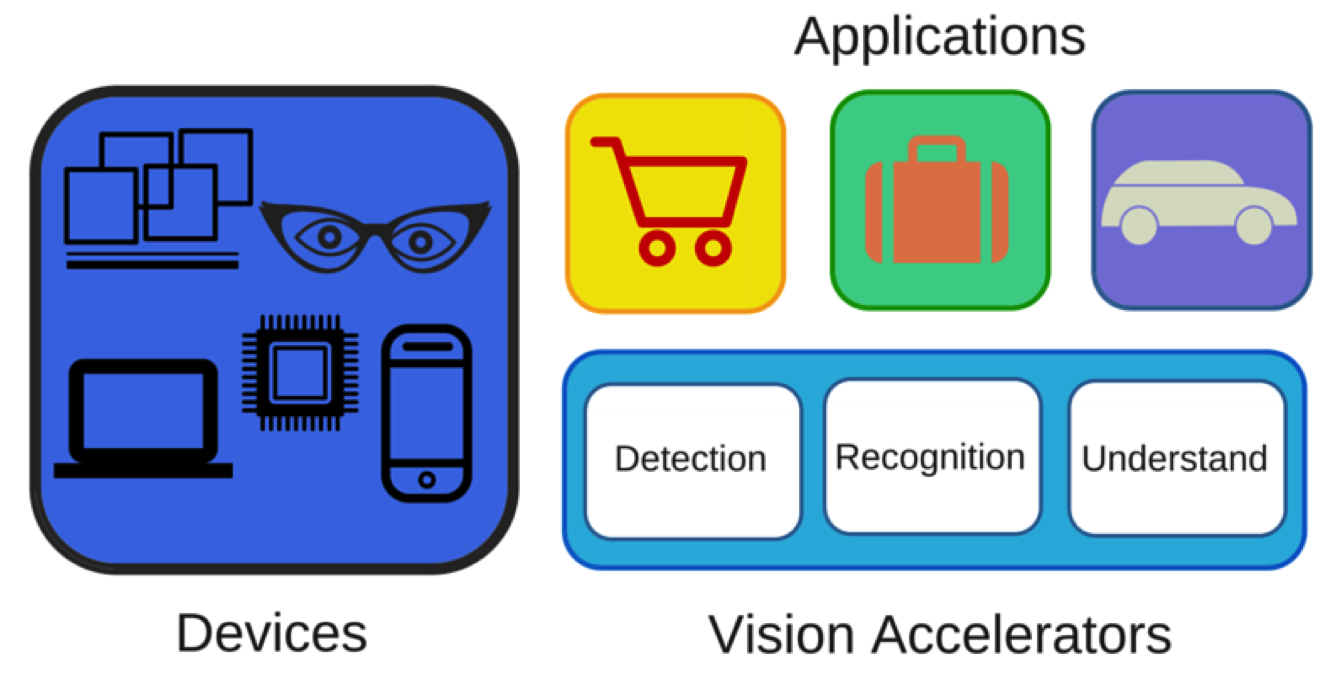
\includegraphics[width=0.9\linewidth]{./figures/vision_apps_devices.png}
\vspace{0pt}
\caption{An embedded vision system consisting of a detection-recognition-understanding pipeline. Regions of Interest (RoIs) are produced from the input visual scene in the detection stage. These RoIs are fed to a recognition system. Having classified these RoIs, more information can be harnessed using more complex vision processes for scene understanding.}
\label{fig:iot}
\vspace{0pt}
\end{figure}

Fig.~\ref{fig:iot} illstrates the interaction between compute devices and vision accelerators when targeting various applications. A common vision pipeline involves parsing the visual scene and extracting objects or regions of interest (RoIs). This is 
carried out in the object detection stage. Once regions are extracted they are sent to a recognition stage to identify 
what the object is. Having figured out whether the object is of interest, further options can be explored. For example, if the 
object is a person, activity or pose estimation can be triggered. The application workload usually will decide the choice of 
the compute device. For example, if a user is in a retail store and would like to use a smart visual-assist device, a 
wearable small form-factor device would be ideal. However, if this is an automotive-assist system, a larger device may be 
engaged. If a security application is being deployed at an airport, then a large server-scale architecture would be needed to
handle the sheer volume of data being generated every minute. It should be noted that in all these applications, real-time is a necessary constraint that needs to be met by the underlying system.

In the context of real-time vision applications, object detection is a highly computationally intensive task.  
To robustly detect an object
in an image that may appear at arbitrary position and scale involves (1) extracting optimized features that aptly describe the object and (2) 
searching the image in a sliding window fashion for the presence of particular configurations of the features that are indicative of the object's presence. 
This exhaustive search is compounded by objects that exhibit high appearance variability in shape, color and size. 
But, for visual-assist systems, the ability to perform such a task is imperative. For example, in a visual driving
assist system, an approaching vehicle or a passing pedestrian needs to be detected
with minimal latency, minimum false positives, and maximum accuracy. On the other hand, a wearable visual prosthesis device needs to augment the visual cognition of the user 
in diverse and vastly unconstrained environments for extended periods of time.

The main contributions of this paper are:
\begin{itemize}
\item To usher in the next wave of technology, we explore the current state-of-the-art in 
embedded vision accelerators and lay emphasis on key insights when designing such accelerators.
\item With scaling technology paving the way for approximate computing, we exploit an increasingly powerful property of most vision algorithms - reliability to noise. 
We show that for an object recognition system, we can save upto X\% refresh power when using DRAMs for memory storage while maintaining a 1\% error bound on accuracy.
\end{itemize}

The rest of this paper is organized as follows:
In Section~\ref{sec:related}, we provide an overview of vision-based architectures and the corresponding state-of-the-art.
Section~\ref{sec:reliability} describes a robust object recogntion pipeline.
Finally, we conclude with Section~\ref{sec:conclusion}.


